\chapter{Introduction} \label{introduction} 
%El proposito de este trabajo de investigacion es para aportar en las 
The purpose of this research is to contribute in the diverse forms of use of the interactive learning environments 
%diversas formas de uso de los ambientes de aprendizaje interactivos proponiendo un ambiente de aprendizaje 
by proposing a learning environment, we based the content management with an adaptive hypermedia approach and 
%interactivo basado en hipermedia adaptativo y con el desarrollo
% de un nuevo tipo de objeto de aprendizaje para que se adaptara al ambiente de aprendizaje.
with the development of a new type of learning object to be adapted to the learning environment.
%Este ambiente utilizo diversos dispositivos que era capaces de correr un navegador web, se
% utilizaron bases de datos no relacionales para intercambio de informaci�n y algunos sensores como c�maras y Kinect 2.
This environment use various devices that were capable of running a web browser, non-relational data bases for information exchange and some sensors like cameras and Kinect 2 were used. In addition we implemented a way to predict the level of user attention
which it was compared against information obtained by a video taken from the user doing the activity.
%Se realizaron varios experimentos con usuarios reales los cuales utilizaban el ambiente
% donde se obten�a informaci�n v�a encuestas, observaci�n y a trav�s de los sensores. 
%Adem�s implementamos una forma de pronosticar el nivel de atenci�n del usuario 
%la cual fue comparada contra la informaci�n obtenida por un video tomado al usuario realizando la actividad.
\section{Motivation}
A los ambientes de aprendizaje comunmente los asociamos con aulas de escuelas, museos, y lugares parecidos, con las aparicion de nuevas tecnologias los ambientes de aprendizaje estan en evolucionando con ellas como pizzarones interactivos, la evolucion misma de las computadoras, los smart-phones, tablets, sensores y muchas cosas mas.
According to Phillips\cite{PhilMcNaKenn2010zx} a learning environment is a place where resources, time and reasons are available for a group of people to nurture, support and value the learning of a limited set of information. The LE are social places even when only one person is found there. One of the challenges facing the design of learning environments is human complexity, because each person thinks and assimilate information in different ways making it difficult to identify which resources are adequate for everyone. Intelligent learning environments (ILE) are a new type of intelligent educational system, which combines characteristics of traditional intelligent tutoring systems (ITS) \cite{john1991} and learning environments. According to Self \cite{self1998} ITS are learning systems based on computers that try to adapt to the needs of the learner. \\

\begin{figure*}
\captionsetup{font=footnotesize} \centering
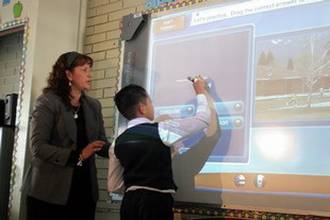
\includegraphics[width=0.5\textwidth]{img/pizzarra.png}  
\small
\caption{Kid interacting with an Electronic Whiteboard}
\label{fig:witheboard}    
\end{figure*} 

ITS research is the only one of the IT's in general which has as its scientific objective create forms of psychological and social educational knowledge. In some ILEs to motivate the learner, he is placed in realistic contexts and authentic representations of tasks in the real world. Resources are given to the user which will help him do these tasks. The resources in the LE are represented in 2 ways, the first is physically (books, printed images, toys etc.), the other is digitally where devices are used to display images, texts, videos, audios helping to contextualize the activity or the environment itself. Currently there are other devices besides computers that can be used in the LE as Smartphone's, Tablet's, projector's, video game consoles etc. The challenge for LE (as we mentioned before) is to select appropriate resources but must also be a learning sequence that satisfies the user needs and make sense of what is being learned. There are many techniques for establishing learning sequences as \cite{DBLP:conf/um/2003},[14] and [16]. In this case we focus on the simple sequence \cite{ims2012} which has the task of generating a sequence of activities of the subject to be learned by the user. In each of these activities there are precondition rules \cite{ims2012} which serve to make decisions about what to do with activities like hide, show, skip or repeat the activity. The rules require certain values to make these decisions for example when there is an activity that displays information that the user may already know and do not need to see it this activity is skipped or if an activity requires the user to have some age to view it. Fuzzy logic has been previously used in learning environments work as \cite{884142},\cite{DBLP:conf/ifsa/2007-2} the advantage offered by fuzzy logic is that it can work with linguistic variables which take values such as "you are young" and turn it into something measurable as 18 years. We propose to use fuzzy logic on the precondition rules. 